\section{Multi-Objective Path-Planning}

% add outline page with current section highlighted.
\begin{frame}{Outline}{ $ \null $ }
	\tableofcontents[currentsection]
	%\tableofcontents[currentsection,currentsubsection]
\end{frame}

\subsection{Algorithm}

\begin{frame}{Multiple Objectives in a Task}{Multi-Objective Path-Planning}
With different objectives, there are different ``best'' paths.
\begin{columns}
\column{0.45\textwidth}
	\begin{figure}
		\centering
		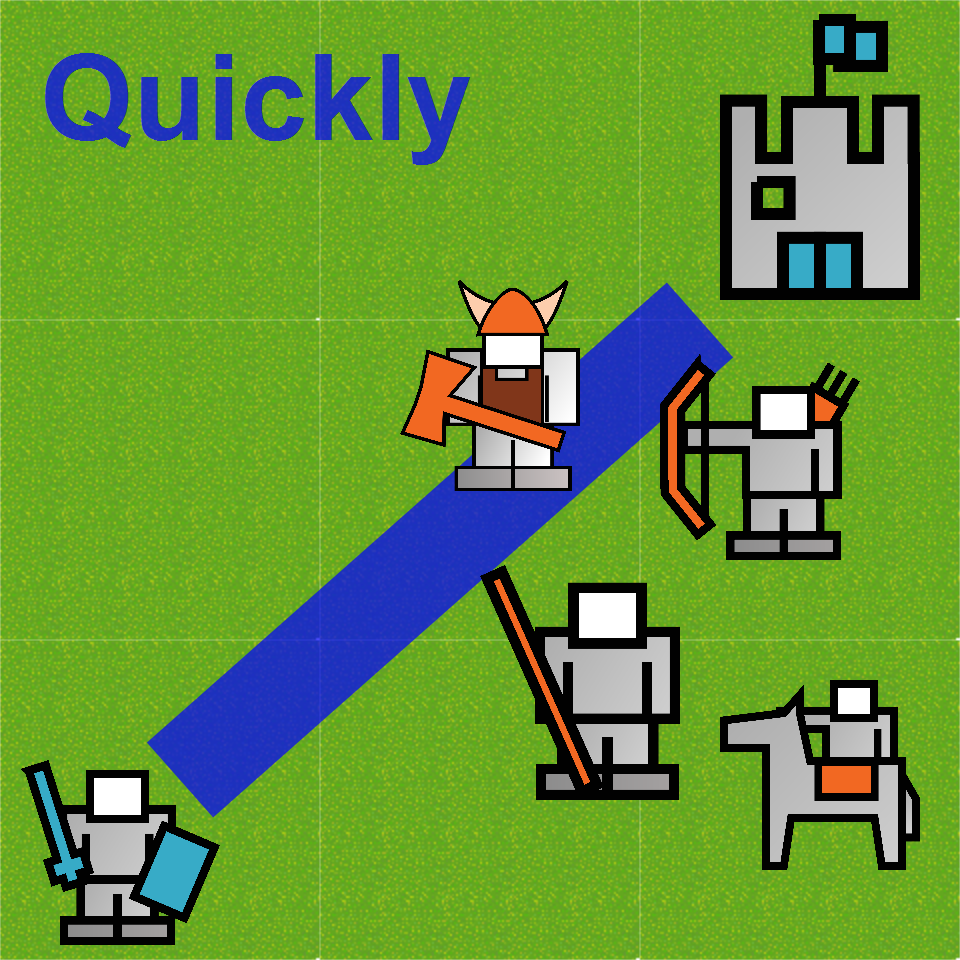
\includegraphics[width=.8\linewidth]{figure/MULTI_OBJ-QUICK}
	\end{figure}
\column{0.45\textwidth}
	\begin{figure}
		\centering
		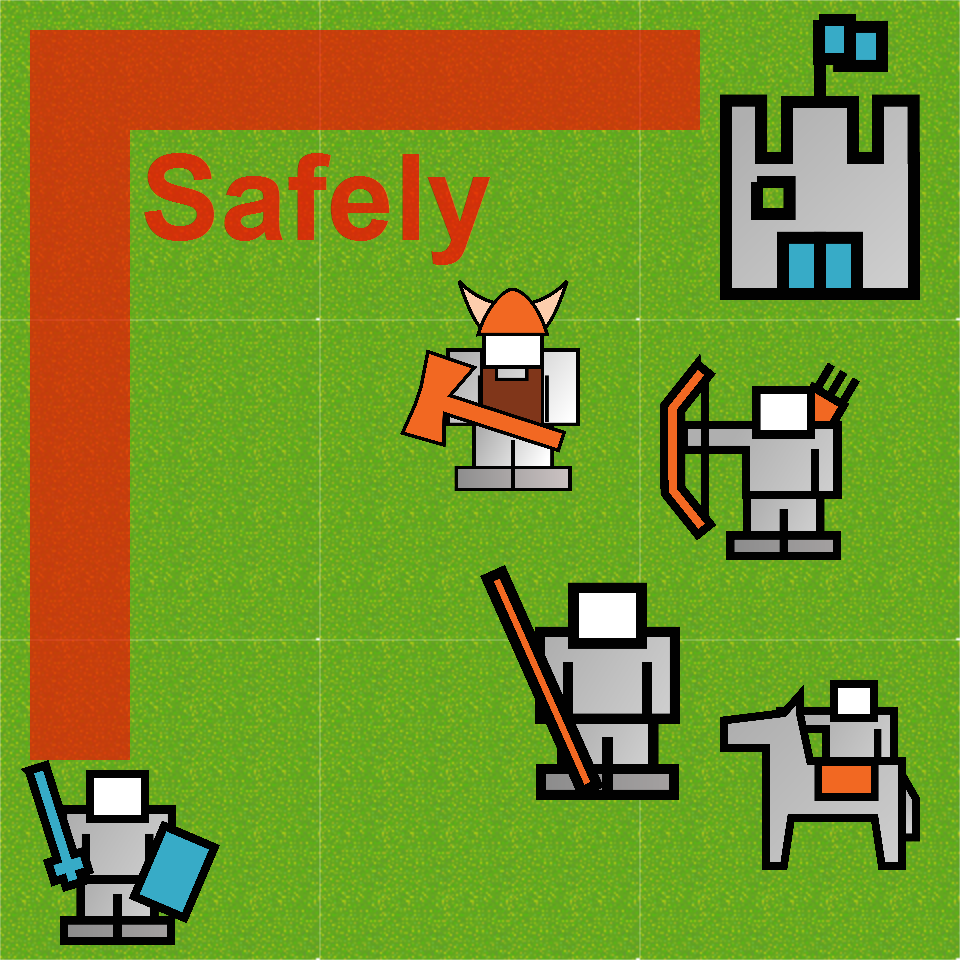
\includegraphics[width=.8\linewidth]{figure/MULTI_OBJ-SAFE}
	\end{figure}
\end{columns}

\end{frame}

\begin{frame}{Multi-Objective Path Planning}{Multi-Objective Path-Planning}
	
	\begin{figure}
		\centering
		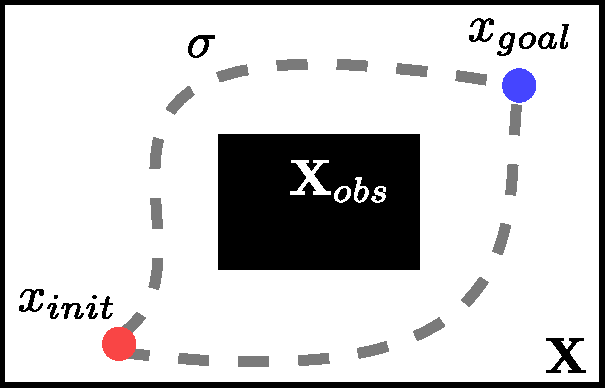
\includegraphics[width=.5\linewidth]{figure/PathPlanning.pdf}
	\end{figure}
	
	\textbf{problem} \\
	\begin{itemize}
		\item \textcolor{reference_color}{$K$ objectives}  $ \bm{c}(\cdot) = [ c_{1} (\cdot), \ldots , c_{K}(\cdot) ]^{T}$ 
		\item find \textcolor{subproblem_color}{$ M $ Pareto optimal paths} $ \sigma^{*} \in \Sigma^{*}$    
	\end{itemize}                        
	
\end{frame}

\begin{frame}{Structure}{Multi-Objective Path-Planning}
	
	{\large \bf {\em M}ulti-{\em O}bjective {\em R}apidly exploring {\em R}andom {\em F}orest$^{*}$}
	
	\begin{center}
		{\large consists of} 
	\end{center}
	
	\begin{columns}
		\column{0.45\textwidth}
		{\Large \bf \textcolor{reference_color}{$ K $ reference trees}}
		\column{0.1\textwidth}
		{\Large + }
		\column{0.45\textwidth}
		{\Large \textcolor{subproblem_color}{$ M $ subproblem trees}}
	\end{columns}
	
	\begin{columns}
		\column{0.5\textwidth}
		\setbeamercolor{block title}{use=structure,fg=white,bg=reference_color}
		\begin{block}{\bf Reference tree}
			\begin{itemize}
				\item From {\em $ K $ objectives}
				\item Each tree serves one objective
				\item Supporting the Utopia reference vector
			\end{itemize}	
		\end{block}
		\column{0.5\textwidth}
		\setbeamercolor{block title}{use=structure,fg=white,bg=subproblem_color}
		\begin{block}{\bf Subproblem tree}
			\begin{itemize}
				\item From {\em $ M $ solutions}
				\item Each tree serves one subproblem (one weight)
				\item This set approximates the Pareto-optimal set
			\end{itemize}
		\end{block}
		
	\end{columns}
	
\end{frame}

\begin{frame}{Process}{Multi-Objective Path-Planning}
	\begin{figure}
		\centering
		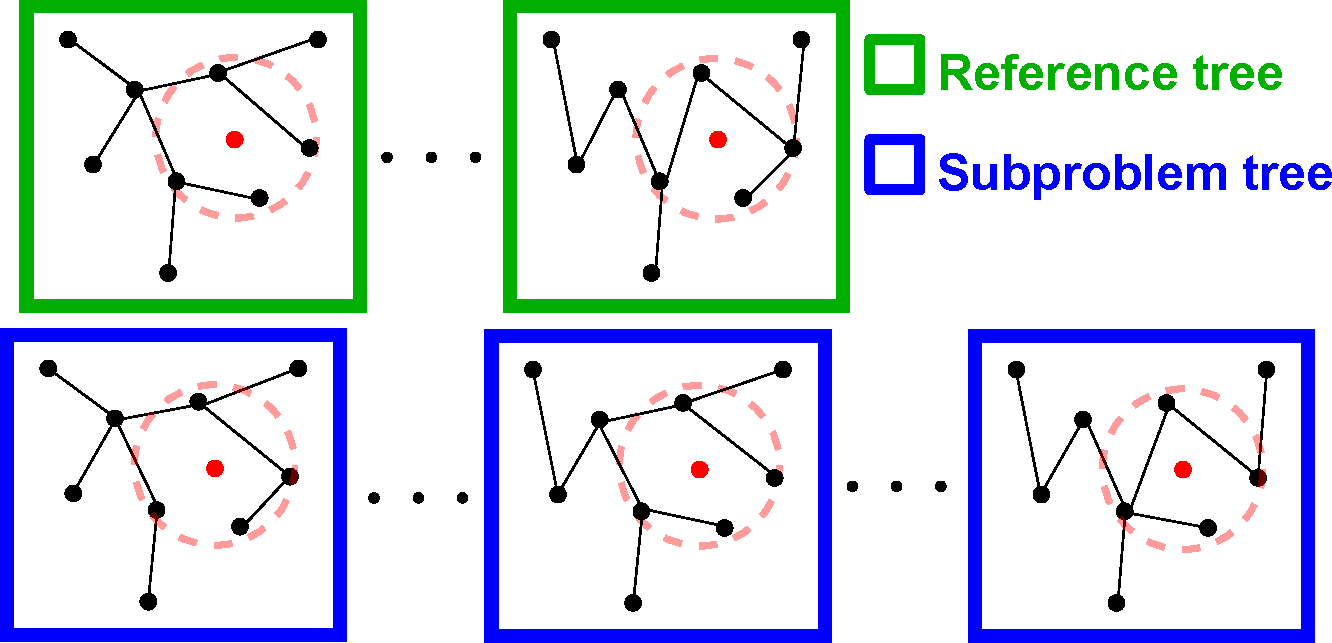
\includegraphics[width=.7\linewidth]{figure/morrf.pdf}
		%\caption{}
		\label{fig:morrt:process}
	\end{figure}
	\begin{itemize}
		\item All the trees have same vertices.
		\item The vertices are differently connected because of the single-objective function.
	\end{itemize}
	
\end{frame}

\begin{frame}{Approaches}{Multi-Objective Path-Planning}
	
	{\bf Different approaches}
	
	\begin{itemize}
		\item
		\begin{minipage}{0.5\textwidth}
			\begin{block}{}
				\centering
				Weighted-Sum Approach
			\end{block}
		\end{minipage}
		\item
		\begin{minipage}{0.5\textwidth}
			\begin{block}{}
				\centering
				Tchebycheff Approach
			\end{block}
		\end{minipage}
		\item
		\begin{minipage}{0.5\textwidth}
			\begin{block}{}
				\centering
				Boundary-Intersection Approach
			\end{block}
		\end{minipage}
	\end{itemize}
	
	
\end{frame}

\begin{frame}{Weighted-Sum Approach}{Multi-Objective Path-Planning}

	{\bf Weighted-Sum Approach}
	
	\begin{columns}
		\column{0.4\textwidth}
		\begin{figure}[t]
			\centering
			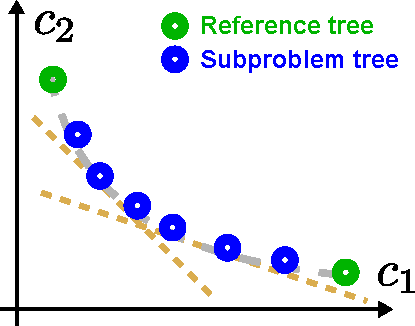
\includegraphics[width=\linewidth]{figure/MORRF_weighted_sum}
		\end{figure}
		\column{0.57\textwidth}
		
        \begin{block}{}
		\begin{equation}
		\nonumber
		\arg\min_x \sum_{k=1}^{K} \lambda_{k} c_{k} (x)
		\end{equation}
		\end{block}

		
		\footnotesize{
			\begin{itemize}
			    \item Each reference tree returns a solution of one objective.
				\item Each subproblem tree returns a solution of weighted sum of all the objectives.
			\end{itemize}
		}
	\end{columns}
	
\end{frame}

\begin{frame}{Tchebycheff Approach}{Multi-Objective Path-Planning}
	{\bf Tchebycheff Approach}
	\begin{columns}
		\column{0.4\textwidth}
		\begin{figure}[t]
			\centering
			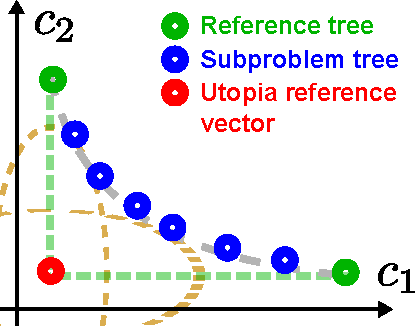
\includegraphics[width=\linewidth]{figure/MORRF_tchebycheff}
		\end{figure}
		\column{0.57\textwidth}
		
        \begin{block}{}
		\begin{equation}
		\nonumber
		\arg\min_x\max_{1 \leq k \leq K}  \{ \lambda_{k} | c_{k}(x) - \bm{z}^{\rm utop}_{k}  | \}
		\end{equation}
		\end{block}

		
		\footnotesize{
			\begin{itemize}
				\item Each reference tree adds a new vertex.
				\item Support the Utopia reference vector of the new position.
				\item According to the estimated Utopia reference vector, each subproblem tree adds a new vertex correspondingly.
			\end{itemize}
		}
	\end{columns}
\end{frame}

\begin{frame}{Boundary-Intersection Approach}{Multi-Objective Path-Planning}
	{\bf Boundary-Intersection Approach}
	\begin{columns}
		\column{0.4\textwidth}
		\begin{figure}[t]
			\centering
			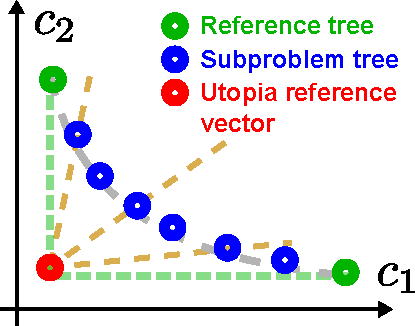
\includegraphics[width=\linewidth]{figure/MORRF_boundary_intersection}
		\end{figure}
		\column{0.57\textwidth}
		
        \begin{block}{}
		\begin{equation}
		\nonumber
		\arg\min_x \{ d \mid \bm{z}^{\rm utop} - c(x) = d \bm{\lambda} \} 
		\end{equation}
		\end{block}

		\footnotesize{
			\begin{itemize}
				\item Each reference tree rewires vertices near the new vertex.
				\item Support the Utopia reference vector of the rewired positions.
				\item According to the estimated Utopia reference vector, each subproblem tree rewires vertices near the new vertex correspondingly.
			\end{itemize}
		}
	\end{columns}
\end{frame}

\begin{frame}{Algorithm}{Multi-Objective Path-Planning}

	\begin{figure}[t]
		\centering
		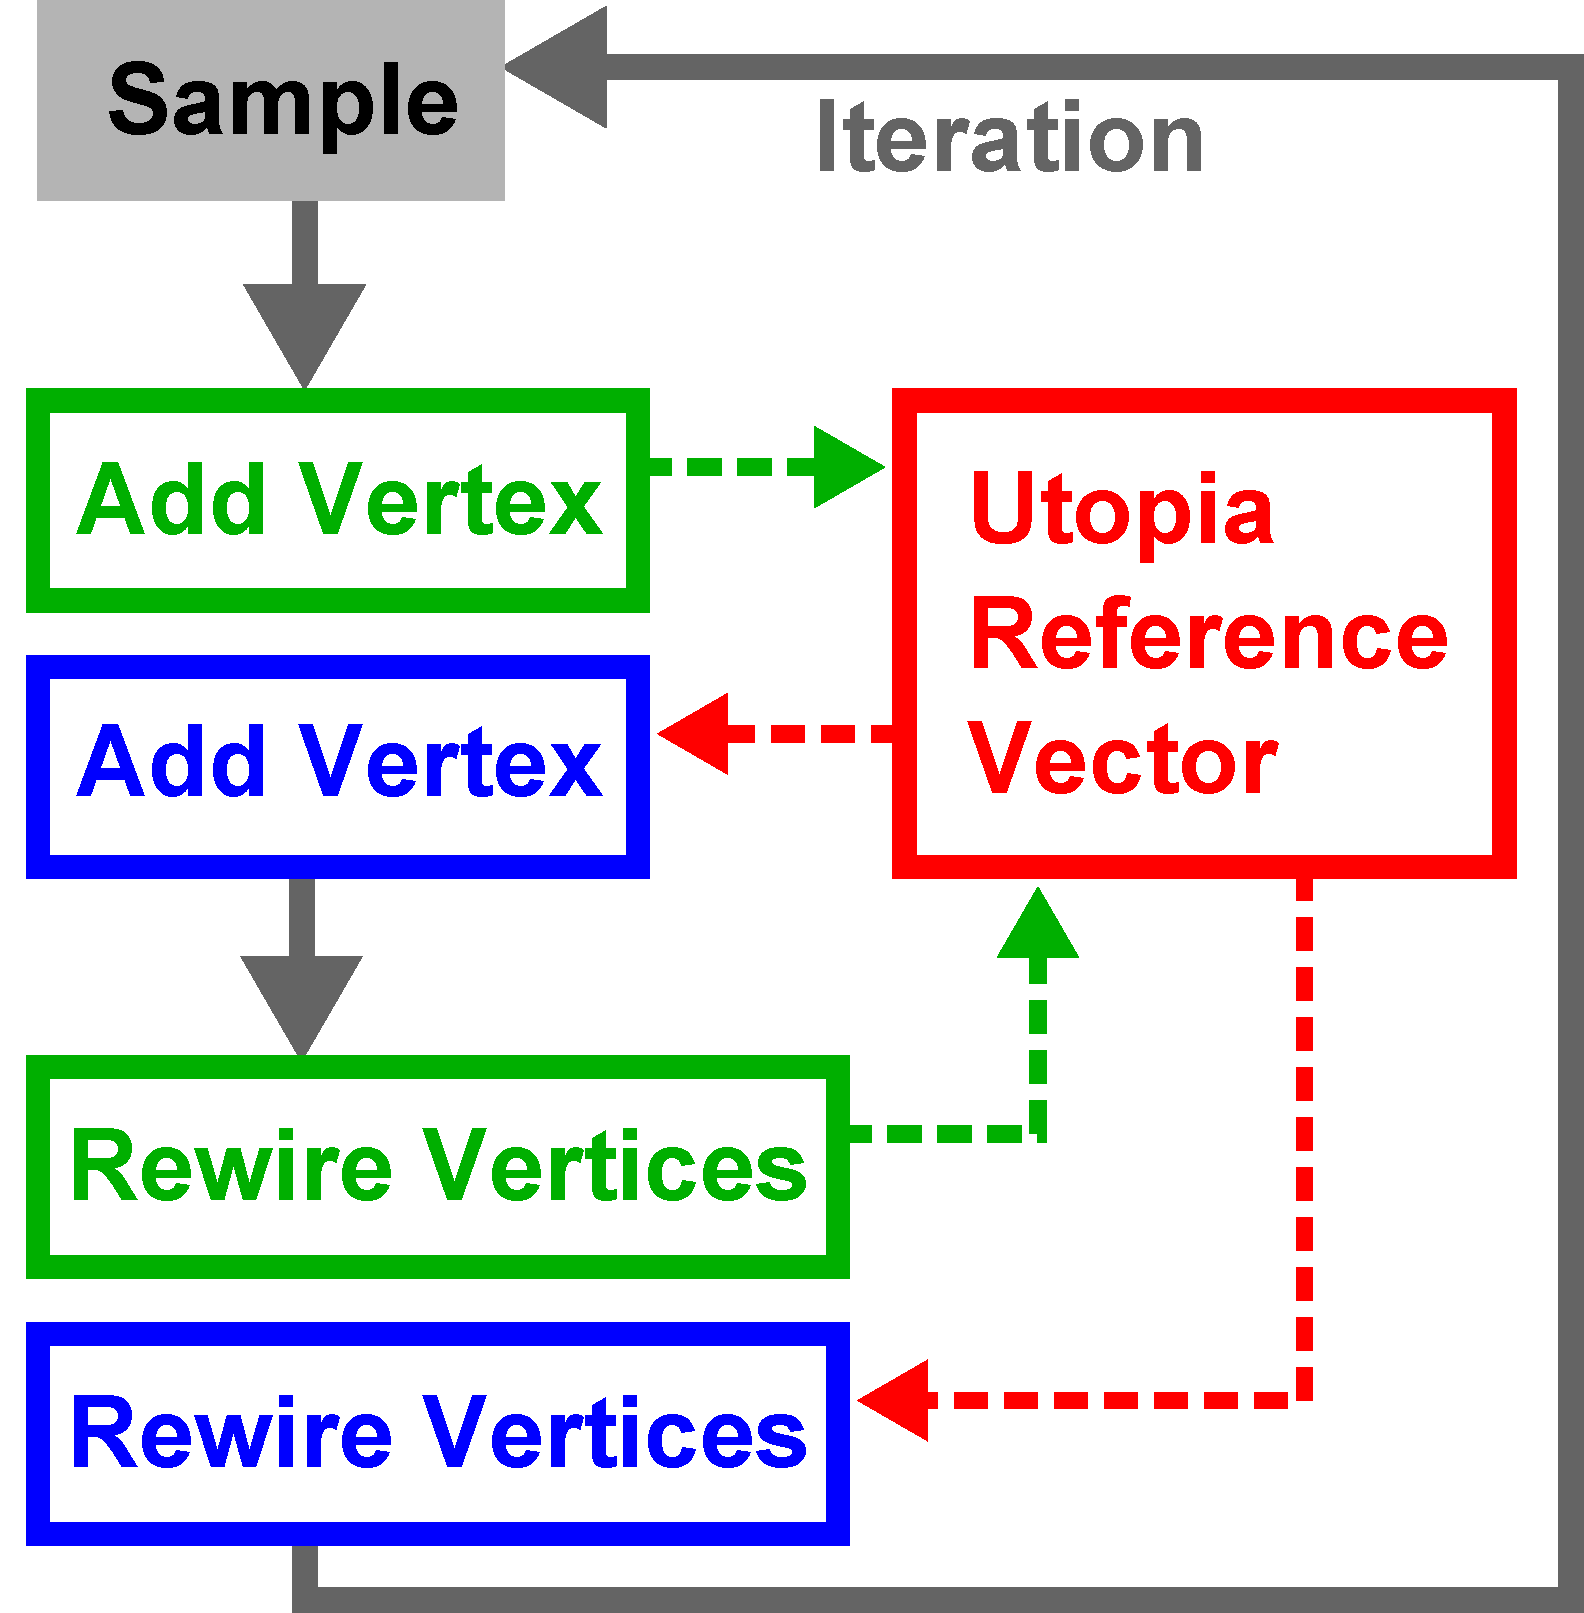
\includegraphics[width=.5\linewidth]{figure/MORRF_alg}
	\end{figure}

\end{frame}

\subsection{Validation}

\begin{frame}{Validation - Theoretical Analysis}{Multi-Objective Path-Planning}

\begin{thm}
	The solutions generated by MORRF$^{*}$ \textcolor{blue}{converge} to \textcolor{red}{a subset of the Pareto optimal set}
	\textcolor{blue}{almost surely}.
\end{thm}

\begin{columns}
\column{0.45\textwidth}
	\begin{figure}
		\centering
		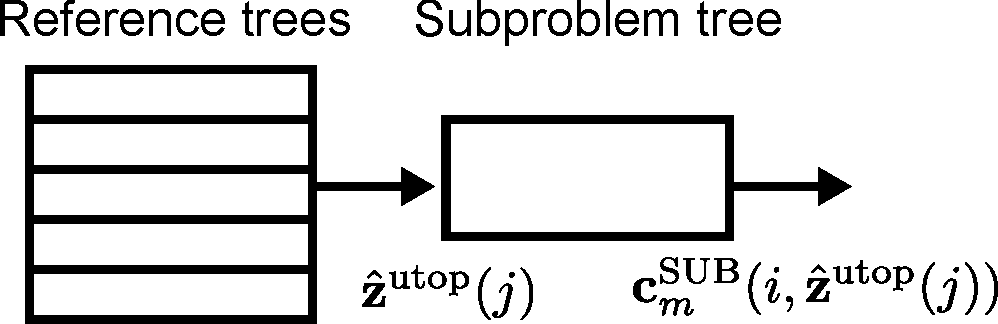
\includegraphics[width=.8\linewidth]{figure/cascade}
	\end{figure}
\column{0.45\textwidth}
	\begin{figure}
		\centering
		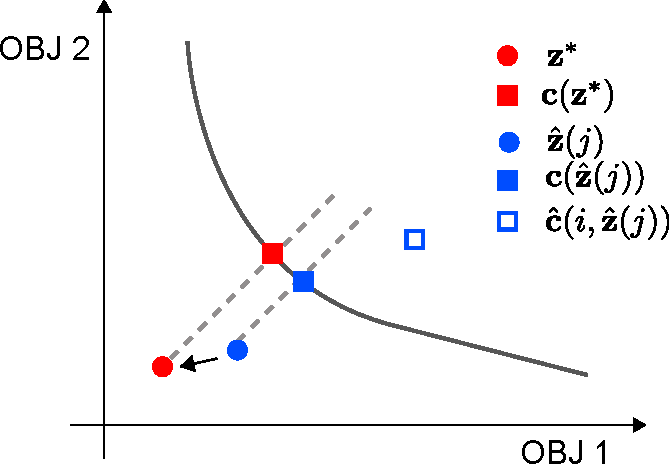
\includegraphics[width=.8\linewidth]{figure/conv}
	\end{figure}
\end{columns}	
	
\end{frame}

\begin{frame}{Validation - Simulation}{Multi-Objective Path-Planning}

\begin{columns}
\column{0.32\textwidth}
	\begin{figure}
		\centering
		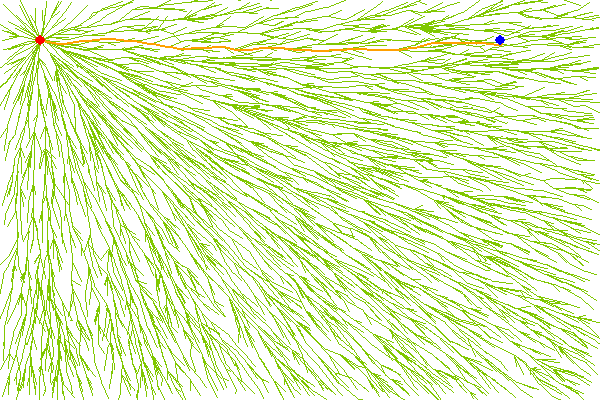
\includegraphics[width=\linewidth]{figure/sim2-2obj/MORRTstar00-0}
	\end{figure}
\column{0.32\textwidth}
	\begin{figure}
		\centering
		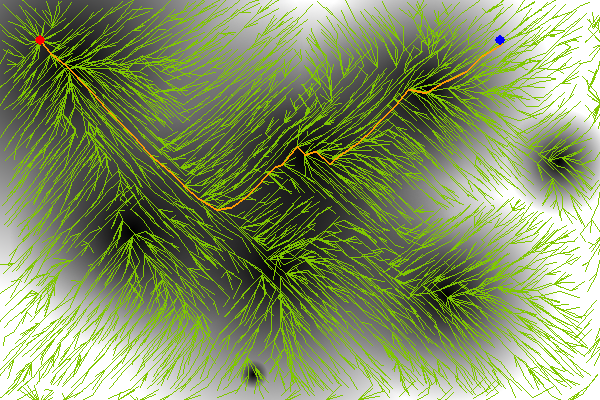
\includegraphics[width=\linewidth]{figure/sim2-2obj/MORRTstar00-1}
	\end{figure}
\column{0.35\textwidth}
\begin{block}{Process}
\begin{itemize}
\item Different cost function
\item Parallel exploration
\end{itemize}
\end{block}		
\end{columns}

\begin{columns}
\column{0.32\textwidth}
	\begin{figure}
		\centering
		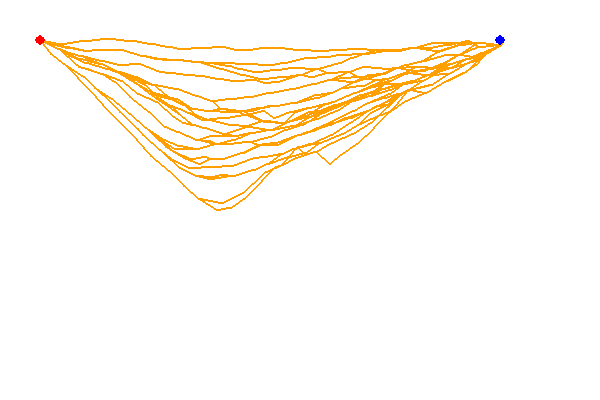
\includegraphics[width=\linewidth]{figure/sim2-2obj/MORRTstar00-ALL}
	\end{figure}
\column{0.32\textwidth}
	\begin{figure}
		\centering
		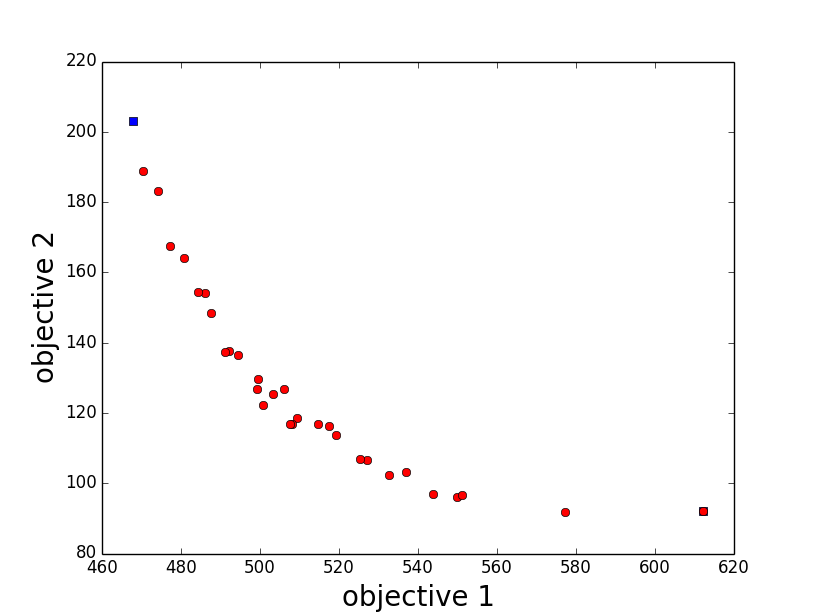
\includegraphics[width=\linewidth]{figure/sim2-2obj/PF02-MORRT2}
	\end{figure}
\column{0.35\textwidth}	
\begin{block}{Performance}
\begin{itemize}
\item Pareto optimality
\item Solution diversity
\end{itemize}
\end{block}	
\end{columns}
	
\end{frame}


\begin{frame}{Validation - Simulation}{Multi-Objective Path-Planning}

\begin{columns}[t]

\column{0.32\textwidth}
\begin{block}{Approaches}
\begin{itemize}
\item NSGA-II
\item Weighted-Sum Approach
\item Tchebycheff Approach
\item Boundary-Intersection Approach
\end{itemize}
\end{block}

\column{0.32\textwidth}
\begin{block}{Environment}
\begin{itemize}
\item Non-Obstacle
\item Obstacle
\end{itemize}
\end{block}

\column{0.32\textwidth}
\begin{block}{Objectives}
\begin{itemize}
\item Two objectives
\item Three objectives
\item Non-convex objectives
\end{itemize}
\end{block}

\end{columns}

\end{frame}
